\chapter{Lab Assignments}

In these labs you can use any programming language that you want. 
In each assignment you must deliver the source code and a brief explanatory pdf document explaining how you solved the assignment.
It should also include some examples, including the commands that you used to test it and the results.
Some assignments may ask for additional information, such as plots.

Pack all the files in a zip file (not rar) and submit it using moodle.
Remember to include the names and NIA in all the source files and in the document.

Prepare the assignment in advance, so that you can complete it during the class.
The submission deadline will be one week after the class.

\section{Traffic Generator and Sink}

In this lab assignment you will program a Poisson traffic generator and a traffic sink.
The Poisson traffic generator takes the following parameters:
destination host, destination port, packet rate and traffic class.

It generates UDP packets with a string that contains three integer values separated by a blank space. The integers represents a packet id (starting with 0), time stamp in milliseconds (local significance only) and traffic class\footnote{Some students reported a mysterious problem disappearing when adding a trailing space}.

The traffic sink takes a port number as a parameter and computes packet delay and packet loss (computation of jitter is optional).

Test it with a traffic generation rate of 10 packets per second.

Note that since the generator and the sink are directly connected, the delay, the jitter and the packet loss will will be zero.

In the next assignment we will place a queue in between.
Then these values will no longer be zero.

\begin{figure}[!h]
\centering
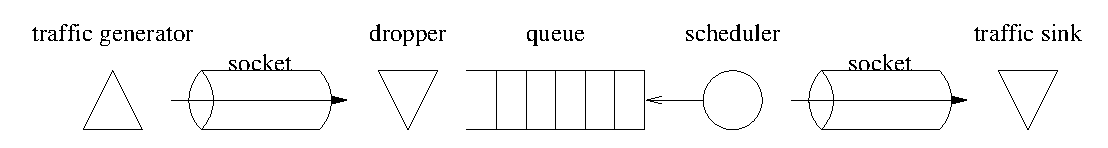
\includegraphics[width=\linewidth]{figures/scenario.eps}
\caption{Scenario to test in lab assignment.}
\label{fig:scenario}
\end{figure}

\section{A queue}

The second module that you have to construct in this course contains a queue (that includes a dropper a buffer) and a scheduler.

Note that each module has to be a separate program. The different modules communicate (send packets to each other) using sockets.

This program listens at an udp port and transmits the packets to a given udp port and address. Consequently, it has to be simultaneously an UDP server and an UDP client. You may consider the possibility of using different threads for the dropper and the scheduler.

All port numbers and the destination should be configurable as parameters. An additional parameter will configure the queue size (number of packets). If the queue size is set to zero, it means infinite queue length. If a finite queue is used, a taildrop policy will be applied.

The scheduler should be configurable to be able to choose an exponentially distributed service time or a deterministic service time. In either case, the service rate should be taken as an input parameter.

Combine the Buffer with the traffic generator and traffic sink modules to make measures of packet loss and delay.

Prepare a plot comparing the packet delay and packet loss obtained from the simulation and theoretical results.

\begin{figure}[!h]
\centering
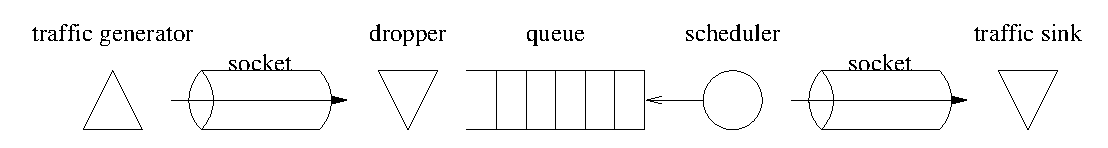
\includegraphics[width=\linewidth]{figures/scenario2.eps}
\caption{Scenario to test in lab assignment 2.}
\label{fig:scenario2}
\end{figure}

\section{Priority Queues}
The third module that you have to construct in this course contains two priority queues (that include a dropper a buffer) and a scheduler.
We will name $H$ the high priority queue and $L$ the low priority queue.

Each module has to be a separate program. The different modules communicate (send packets to each other) using sockets.

This program listens to two udp ports and transmits the packets to a given udp port and address. Consequently, it has to be simultaneously an UDP server and an UDP client. You may consider the possibility of using different threads for the droppers and the scheduler.

The scheduler strictly prioritizes queue $H$.
That is, it starts to serve queue $L$ only if there are no packets at queue $H$.
Nevertheless, this is non-preemptive priority, which means that the server will not interrupt a service to queue $L$ when a packet arrives to queue $H$.
The server will complete the service to the packet of queue $L$ and only then it will serve the packet that has arrived to queue $H$.

All port numbers and the destination should be configurable as parameters. An additional parameter will configure the queue size (number of packets). If the queue size is set to zero, it means infinite queue length. If a finite queue is used, a taildrop policy will be applied.

The scheduler will draw service times from an exponential distribution.

Combine the priority queues with two traffic sources that generate different classes of traffic and obtain statistics of the delay for each of the traffic classes.

Prepare a plot combining analytical results and simulation results.

\begin{figure}[!h]
\centering
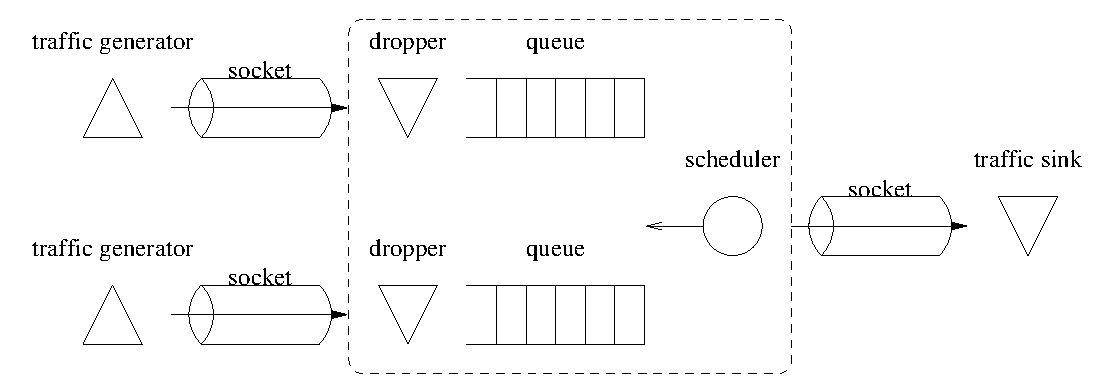
\includegraphics[width=\linewidth]{figures/scenario3.eps}
\caption{Scenario to test in lab assignment 3.}
\label{fig:scenario3}
\end{figure}

\section{Optional QoS Tool}

In this lab assignment you will implement one ore more QoS tools of your choice.
You can choose any of the tools that we have seen in class, e.g.,  classifier, metering, token-bucket policer, (weighted) RED, weighted taildrod, re-write.

A brief description of each of the tools follows:
\begin{itemize}
  \item{classifier:}
  It has an input socket and several output sockets (one for each possible class of service).
  The classifier checks the class of server marking of the packet and redirects the packet accordingly.
  \item{metering:}
  It has an input socket and three output sockets.
  It uses two token buckets (as described in rfc2698) and it takes as an input four parameters: CIR (packets per second), PIR (packets per second), CIR burst (packets) and PIR burst (packets).
  The green, yellow and red packets are sent to each of the three different output sockets.
  \item{token-bucket policer:}
  It takes two parameters: rate (packets per second) and burst size (packets).
  Non-compliant packets are discarded.
  \item{ RED}
  It takes a rate and a size as input parameters.
   The probability of dropping an arriving packet is equal to the occupancy of queue at the moment of arrival.
  \item{Weighted taildrop }
  It takes a rate and a size as input parameters.
  The queue only accepts high priority packets when the queue is half-full.
   The probability of dropping an arriving packet is equal to the occupancy of queue at the moment of arrival.
  \item{re-write}
  It changes the class field of the packet.
\end{itemize}

Another option is to implement queueing disciplines from the ones that we have seen in class (e.g., weighted round robin, weighted fair queueing and deficit weighted round robin)

The idea is that different groups implement different tools.
Keep in mind that in the next (last) lab assignment you should combine your tool and some of your classmate's tools to create a QoS scenario in which different service classes will receive a different treatment.
You may first think about your scenario and then choose the tool you want to implement accordingly.

%The complexity of metering, token-bucket policer and leaky bucket shaper with RED is considerably higher than the other options.
%It is highly recommended that each group implements at least one of these three tools.

\section{Design and evaluate your own scenario}

This is a free assignment.
With all the knowledge gathered throughout the course and all the developed code, you have to invent an scenario and implement some sort of QoS.

You have to include some invented motivation.
As an example, it may be your home network in which your flat mate is downloading a linux distribution while you are playing an interactive real-time online game.
The download is generating one thousand packets per second and is filling the buffers while the game generates only 10 packets per second and is suffering excessive delays.

You can use different combinations of tools that we have seen and developed during the course.
You can try different parameter configurations (queue length, burst size, rates, different kinds of RED, etc.) and report the results obtained with each of them.
Offer an expert recommendation about which is the best solution and why.

You can also combine and use the queueing theory techniques that we have seen in class, if you wish.

You will have to prepare a presentation (5-10 minutes) to explain your classmates about your project (motivation, possible solutions, test plan, etc.).
Additionally, when you have performed all the tests and computations, you will have to deliver a short report (max. 5 pages) detailing your work.

You can also use code generated by other groups.
Include the slides, the report and all the used code in one zip file that will be submitted via moodle.
Make sure to clarify which code has been generated by you and which code has been developed by other groups and re-used in your project.

